\documentclass[border=3pt,tikz]{standalone}
\usetikzlibrary{arrows}
\usetikzlibrary{positioning}
\usetikzlibrary{calc}
\usetikzlibrary{arrows}
\usetikzlibrary{decorations.pathreplacing}
\begin{document}
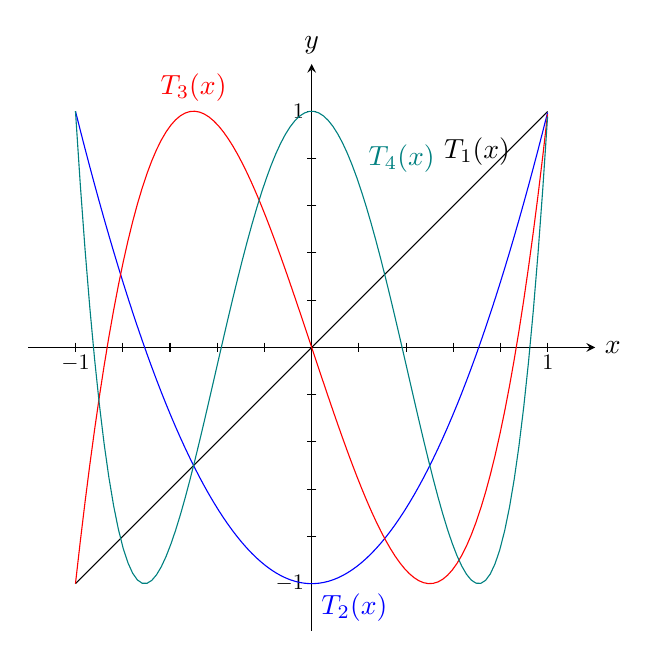
\begin{tikzpicture}[domain=-1:1, samples = 100, scale=3]

    \draw[-{stealth}] (-1.2, 0) -- (1.2,0) node[right] {$x$};
    \draw[-{stealth}] (0,-1.2) -- (0,1.2) node[above] {$y$};
    \node[left, scale=0.8] at (0, 1) {$1$};
    \node[left, scale=0.8] at (0, -1) {$-1$};
    \node[below, scale=0.8] at (-1, 0) {$-1$};
    \node[below, scale=0.8] at (1, 0) {$1$};
    
    \foreach \x in {-5,...,5}
    {
      \draw[thin] (\x / 5, 0.02) -- (\x /5, -0.02);
      }
    
    \foreach \y in {-5,...,5}
    {
      \draw[thin] (0.02 , \y / 5) -- (-0.02 , \y /5);
      }
    
    \draw[color=black]   plot (\x, \x) ;
    \node[above, black] at (0.7, 0.73) {$T_1(x)$};
    \draw[color=blue]   plot (\x, 2 * \x * \x - 1);
    \node[below right, blue] at (0, -1) {$T_2(x)$};
    \draw[color=red]   plot (\x, 4 * \x * \x * \x - 3* \x);
    \node[above, red] at (-0.5, 1) {$T_3(x)$};
    \draw[color=teal]   plot (\x, 8 * \x * \x * \x * \x - 8* \x * \x + 1);
    \node[right, teal] at (0.2, 0.8) {$T_4(x)$};
    \end{tikzpicture}
\end{document}